\fontfamily{\sfdefault}\selectfont
% XCircuit output "quantization.tex" for LaTeX input from quantization.ps
\def\putbox#1#2#3#4{\makebox[0.00000in][l]{\makebox[#1][l]{}\raisebox{\baselineskip}[0.00000in][0.00000in]{\raisebox{#2}[0.00000in][0.00000in]{\scalebox{#3}{#4}}}}}
\def\rightbox#1{\makebox[0.00000in][r]{#1}}
\def\centbox#1{\makebox[0.00000in]{#1}}
\def\topbox#1{\raisebox{-0.60\baselineskip}[0.00000in][0.00000in]{#1}}
\def\midbox#1{\raisebox{-0.20\baselineskip}[0.00000in][0.00000in]{#1}}
   \scalebox{1}{
   \normalsize
   \parbox{4.24010in}{
   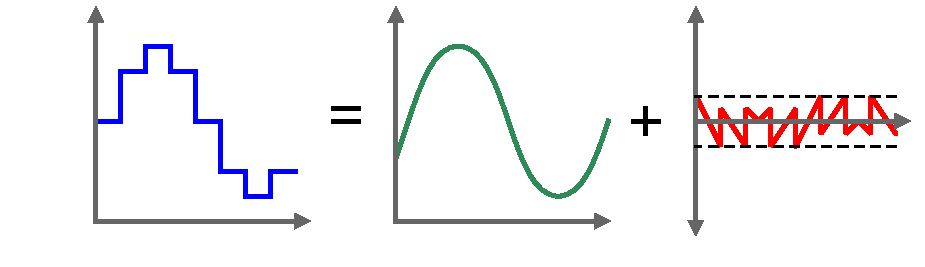
\includegraphics[scale=0.70000]{./figs/quantization.pdf}\\
   % translate x=304 y=240 scale 0.38
   \putbox{0.04200in}{1.09200in}{0.96}{$e_\Phi$[n]}%
   \putbox{1.32300in}{0.04200in}{0.96}{t=nT}%
   \putbox{1.32300in}{1.09200in}{0.96}{$\frac{\mathrm{M}}{2\pi}\Phi_e$[n]}%
   \putbox{2.77900in}{0.04200in}{0.96}{\rotatebox{-360}{t}}%
   \putbox{4.24200in}{0.50400in}{0.96}{t}%
   \putbox{2.72300in}{1.09200in}{0.96}{q$_{\mathrm{TDC}}$[n]}%
   \putbox{3.47900in}{0.85400in}{0.96}{$+\Delta/2$}%
   \putbox{3.47900in}{0.44800in}{0.96}{$-\Delta/2$}%
   } % close 'parbox'
   } % close 'scalebox'
   \vspace{-\baselineskip} % this is not necessary, but looks better
\fontfamily{\rmdefault}\selectfont
